\begin{figure*}[t]
	\centering
	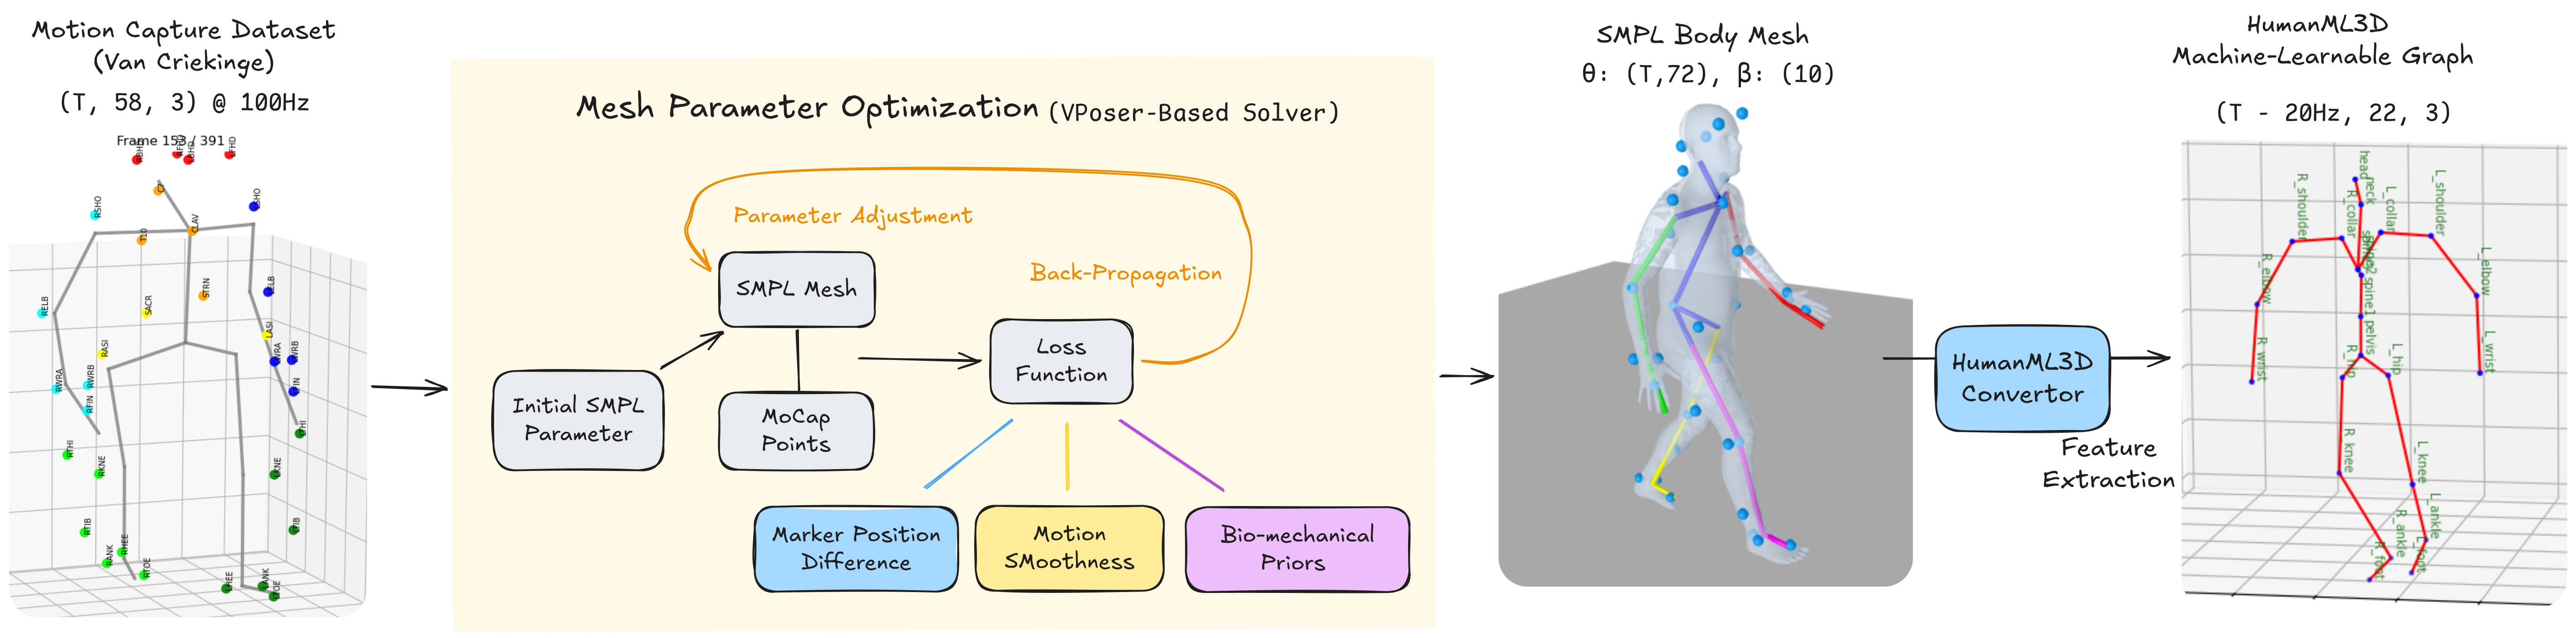
\includegraphics[width=0.7\textwidth]{sec/figs/18 - Data Pipeline Diagram.png}

	\vspace{0.6em}

	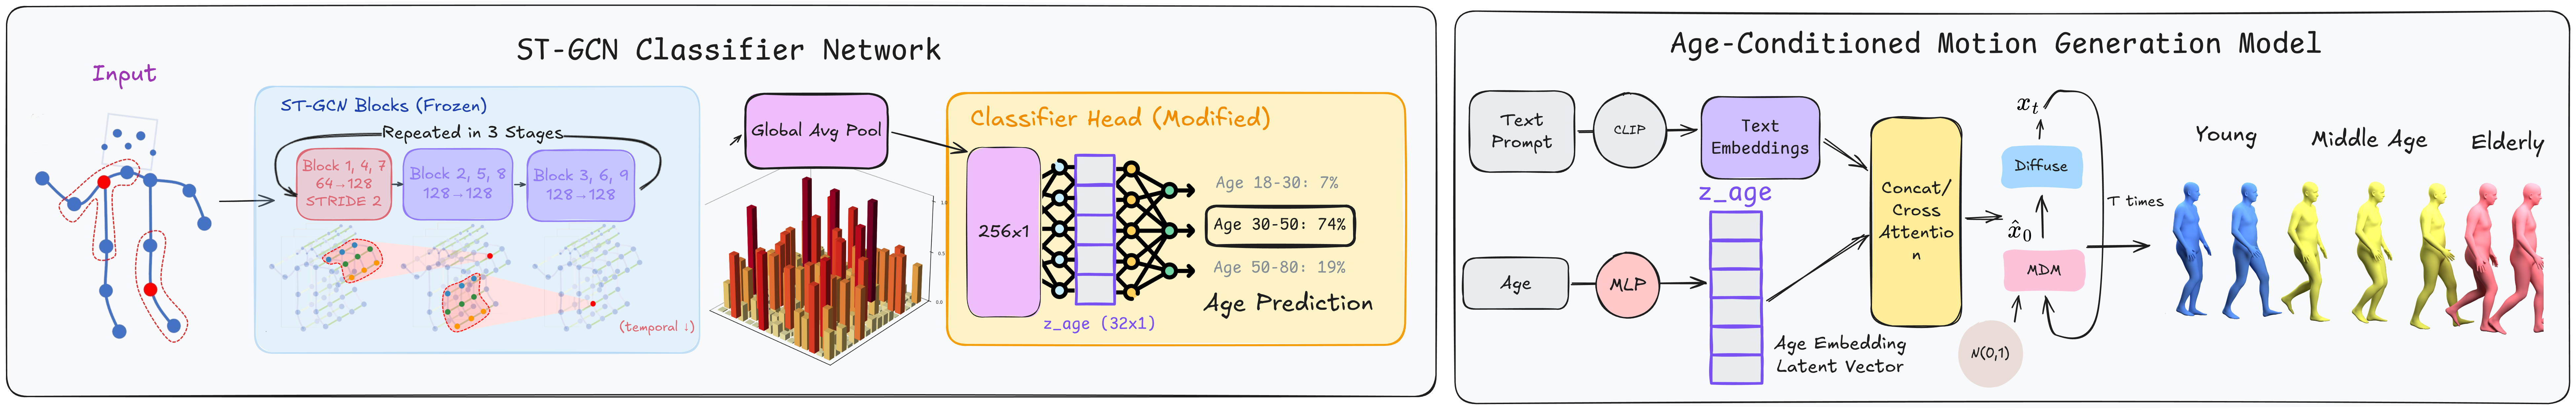
\includegraphics[width=\textwidth]{sec/figs/24 - Revised Motion Generation Model.png}
	\caption{Overview of our age-aware motion synthesis framework. \emph{Top:} clinical marker recordings are converted into the 263-dimensional HumanML3D representation via VPoser-regularized SMPL fitting followed by feature extraction. \emph{Bottom:} an ST-GCN++ age representation learner extracts $\mathbf{z}_\text{age}$ (left) and an age-conditioned Motion Diffusion Model (right) generates text-driven motion.}
	\label{fig:framework}
\end{figure*}

Accurate human motion anticipation is foundational for safe human-robot interaction, especially when robots share space with humans, plan around future movement, or provide proactive assistance.
Recent deep generative architectures, particularly Motion Diffusion Models (MDMs)~\cite{tevet2023human, chen2022mld}, have demonstrated strong capability in synthesizing realistic and diverse human motions.
However, widely used motion-capture datasets such as AMASS~\cite{mahmood2019amass} are heavily biased toward young, healthy actors~\cite{umagami2025intend}, so existing generative models cover diverse actions and styles~\cite{sawdayee2025dance} but rarely capture population-level biomechanical factors such as age~\cite{liao2025shapemovestextdrivenshapeaware}.
This limitation is particularly critical for assistive robots in aging-in-place and eldercare scenarios, where anticipating older adults' movements is essential for safe navigation, timely assistance, and proactive interaction.

Although MDMs are trained for synthesis rather than direct forecasting, they implicitly learn the distribution over plausible future motions --- precisely what a prediction system samples from under partial observation.
Age-conditioning this distribution restricts samples to a demographic-specific manifold, giving downstream forecasters and robot planners priors aligned to the user population they serve.
An age-aware generative prior is therefore a precursor to, rather than a substitute for, motion prediction in eldercare contexts; clinical gait analysis, which has long quantified spatiotemporal aging signatures~\cite{diaz2025evaluating, galasso2024development}, provides the supervision signal needed to build it.

To address this gap, we present a proof-of-concept framework that integrates clinical gait analysis with deep generative modeling toward age-aware human motion synthesis.
We develop a data processing pipeline that converts clinical gait recordings into standardized skeletal representations, fine-tune a Spatial-Temporal Graph Convolutional Network (ST-GCN)~\cite{yan2018stgcn} to infer age group and encode age-related biomechanical characteristics into a latent representation, and train a Low-Rank Adaptation (LoRA)~\cite{hu2022lora} adapter for an MDM to generate text-driven motions conditioned on age group.
We evaluate generated motions with clinical and kinematic gait metrics and against the unadapted MDM under both neutral and elderly-described prompts.
Our analysis shows that the adapted model captures spatial kinematic constraints (reduced hip Range-of-Motion in the Elderly condition) that the unadapted MDM fails to express even when prompted explicitly for old age, but fails to reproduce spatiotemporal consistency: stride variability overshoots clinical baselines, a limitation we attribute to the capacity ceiling of low-rank, discrete-token adaptation.
These findings motivate larger, age-diverse human motion datasets and stronger conditioning mechanisms for downstream motion prediction and assistive robot planning.